% !TeX root = ../presentation.tex

\begin{frame}{Agradecimientos}{Grupo de Nanoplasmónica, DGAPA, CONACyT, y más...}%{Para una 12.5 nm AuNP parcialmente embebida entre un sustrato plano y una matriz}

 \begin{columns}
 \column{.5\textwidth}
    \centering
    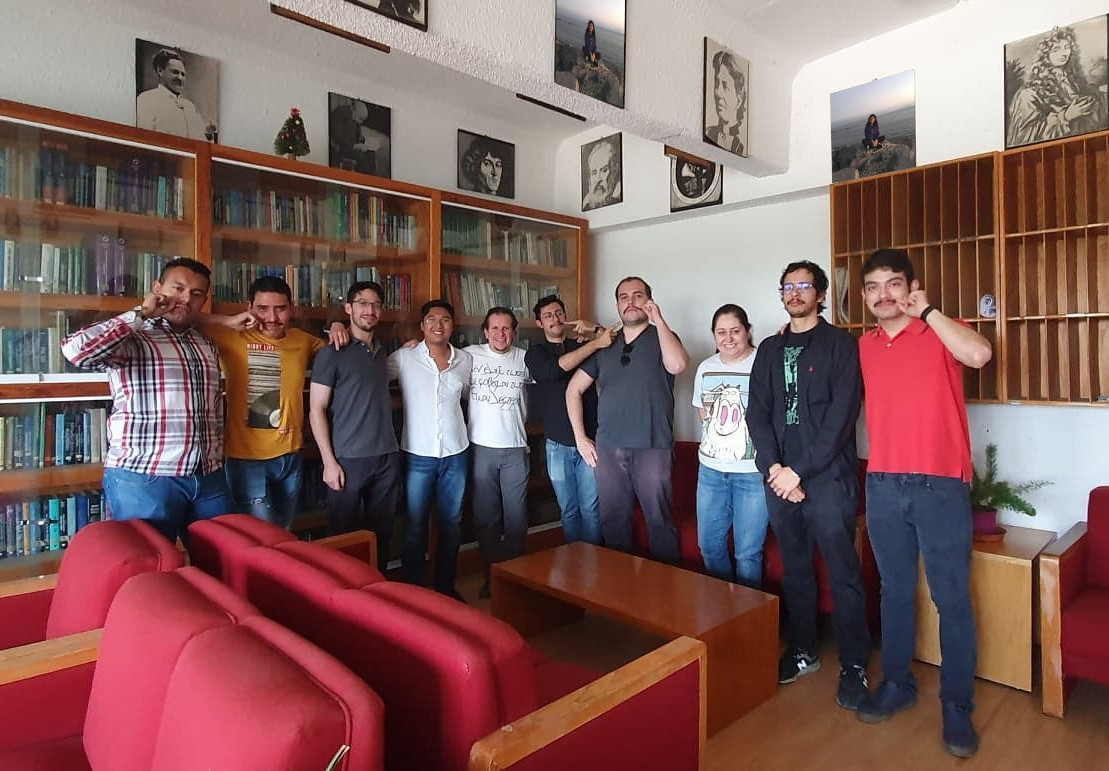
\includegraphics[width = .9\textwidth]{grupo3.jpg}
 \column{.2\textwidth}
 \centering
 \textbf{\large Comité tutor}\\[1em]
       
\includegraphics[width = .45\textwidth]{AReyes.png}\\ {\small Dr. Reyes Coronado}\\[.75em]
        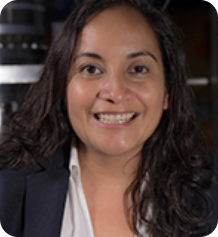
\includegraphics[width = .45\textwidth]{CSanchez.png}\\ {\small Dra. Sánchez Aké}\\[.75em]
         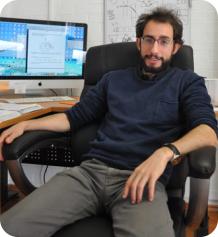
\includegraphics[width = .45\textwidth]{GPirruccio.png}\\ {\small Dr. Pirruccio}
 \column{.3\textwidth}
 \centering
 \includegraphics[width = .6\textwidth]{CONACyT.png}\\[2em]
 
\includegraphics[width = .6\textwidth]{dgapa_unam_azul.png}\\
 {\small PAPIIT IN107122}\\[2em]
 
\includegraphics[width = .4\textwidth]{inaoe.png}
\end{columns}
\end{frame}
